
\chapter{Prosody }
\label{chap:prosody}



\section{Background}
\label{sec:prosody:bg}
\subsection{Prosody, clause types, and speech acts in English}
In English, whether prosody is a surface feature for clause typing or simply an indicator for questioning is debated. English declaratives tend to be associated with falling intonation, polar interrogatives tend to bear rising intonation, while \twh-interrogatives also generally bear a falling contour (\citealt{ladd1981, ladd2008intonational, hedberg2004wh, hedberg2014corpus} among many others). When declaratives are associated with a  L* H-H\% rising intonation, they tend to be interpreted as questions (i.e. rising declaratives, \citealt{ladd1981,gunlogson2004,gunlogson2008,jeong2018,rudin2018,goodhue2021rd}). The main point of contention comes down to whether sentences like (\ref{ex:bg:theory:prosody:rd}) are declaratives or not (I will use $\nearrow$ to indicate the sentence has a final rising intonation, and $\searrow$ for final fall):
 
\bex{ex:bg:theory:prosody:rd}
It's raining $\nearrow$
\eex
\bex{ex:bg:theory:prosody:fd}
It's raining $\searrow$
\eex


In Gunlogson's \cite*{gunlogson2008} analysis, sentences like (\ref{ex:bg:theory:prosody:rd}) are declarative clauses with a rising intonation, implying that intonation does not affect the clause type feature of the sentence. Meaning-wise, clause type and intonation contribute compositionally to the discourse function of the utterance. 


Many analyses of rising declaratives in the dynamic discourse tradition adopt the same assumption. As these cases are rarely discussed in syntactic literature, it is unclear whether syntacticians would classify them as having [$-$int] or [$+$int]. But we can go through
%the arguments given to other
some typical syntactic tests for
[$+$int], to see if it's possible to assign [$+$int] to
%the sentence
rising declaratives. One test is whether rogative verbs that only select interrogative clauses would embed (\ref{ex:bg:theory:prosody:rd}). If (\ref{ex:bg:theory:prosody:rd}) bears [+int], then the sentence with (\ref{ex:bg:theory:prosody:rd}) embedded under \tit{wonder} should be grammatical.

\bex{ex:bg:theory:prosody:rd-wonder}
*Mary wonders \tun{it's raining}.
\eex

As shown in (\ref{ex:bg:theory:prosody:rd-wonder}), this prediction is not borne out; (\ref{ex:bg:theory:prosody:rd}) cannot be embedded under rogative verbs like \tit{wonder}. This suggests that (\ref{ex:bg:theory:prosody:rd}) does not have the feature [+int]. But it could be that (\ref{ex:bg:theory:prosody:rd}) has a silent [+int], but this silent [+int] is realized as \tit{whether} in embedded context. So instead of (\ref{ex:bg:theory:prosody:rd-wonder}), embedded (\ref{ex:bg:theory:prosody:rd}) should be:

\bex{ex:bg:theory:prosody:rd-whether}
Mary wonders \tun{whether it's raining}.
\eex

As the rising intonation associated with (\ref{ex:bg:theory:prosody:rd}) would not manifest in embedded clauses, it's hard to distinguish the two possibilities syntactically. But \textcite{farkasroelofsen2017} observe that if the embedded clause is preposed, the intonation difference is preserved, and rising declaratives pattern with polar interrogatives in these cases:

\bex{ex:bg:theory:prosody:rd-prepose}
\bxl{}
`It's raining$\searrow$,' it appears/*she wondered.
\ex`Is it raining?,' *it appears/she wondered.
\ex`It's raining$\nearrow$,' *it appears/she wondered.
\exl
\eex

\textcite{farkasroelofsen2017} use this evidence to argue that rising declaratives are similar to interrogatives and that this similarity should be captured in part by syntax. They propose that the syntactic representation of sentence forms have two kinds of clause type markers, \tsc{closed/open} and \tsc{dec/int}, as in (\ref{fig:bg:fb2017}). Although they didn't specify where these markers reside in the syntactic structure, but they seem to adopt a split-CP approach following \textcite{rizzi1997}, and thus the two clause markers are both part of CP. 


\begin{figure}[H]
\begin{center}
\begin{tikzpicture}[level distance=30pt]
\tikzset{level 1/.style={sibling distance=15pt}}
\tikzset{level 2/.style={sibling distance=35pt}}
\Tree
[. CP 
	[. \tsc{open/closed} ]
	[. \tsc{}
		[. \tsc{decl/int} ]
		[. TP \edge[roof]; { } ] 
	]
]
\end{tikzpicture}
\end{center}
\caption{Extended structure of CP proposed by \textcite{farkasroelofsen2017}}
\label{fig:bg:fb2017}
\end{figure}

While the morpho-syntax of a sentence is linked to \tsc{dec/int}, the intonation (rise vs. fall) signals whether C bears the feature [\tsc{open}] or [\tsc{closed}]. Rising declaratives like (\ref{ex:bg:theory:prosody:rd}) would be an ``open declarative,'' with the following structure:

\begin{figure}[H]
\begin{center}
\begin{tikzpicture}
\tikzset{level 1/.style={sibling distance=35pt}}
\tikzset{level 2/.style={sibling distance=35pt}}
\Tree
[. CP 
	[. \tsc{open} ]
	[. \tsc{}
		[. \tsc{decl} ]
		[. TP \edge[roof]; {it's raining} ] 
	]
]
\end{tikzpicture}
\end{center}
\caption{The structure of rising declaratives, adapted from \textcite{farkasroelofsen2017}}
\label{fig:bg:fb2017rd}
\end{figure}

So for \textcite{farkasroelofsen2017}, the clause type category of rising declaratives is not exactly declarative with [$-$int] (but rather [\tsc{open,dec}]), and its semantics is similar to that of the polar interrogatives. 

However, as many have noted, there might be two types of rising declaratives. The one discussed in \textcite{farkasroelofsen2017} is the inquisitive one, but there might an assertive one (\cite{jeong2018, goodhue2021rd}), as shown in (\ref{ex:engcl:annt:rd:a}):

\bex{ex:engcl:annt:rd-cont}
\bxl
\label{ex:engcl:annt:rd:q}
\tit{S and A are on their way to a birthday party for the daughter of A’s friend. They stop at a store to get a birthday card. As they are both scanning the display for a card for the correct age, S is trying to remember how old the girl has just turned, and he thinks he remembers A telling him that she just turned nine, but he wants to confirm it.}\\
\tbf{S: She’s nine$\nearrow$}
\ex
\label{ex:engcl:annt:rd:a}
\tit{S is enrolling his daughter in a summer camp program with the camp organizer A.}\\
S: I want to sign her up for Spanish classes in the mornings, and rock climbing in the afternoons.\\
A: Okay, there are limited places in each activity based on age group, and some of the age groups have already filled up for rock climbing. How old is your daughter?\\
\tbf{S: She’s nine$\nearrow$}
\exl
\hspace*{\fill}\hfill ex. (12-13), \cite[955]{goodhue2021rd}
\eex

In (\ref{ex:engcl:annt:rd:q}), the speaker uses the utterance to elicit a confirmation from the addressee regarding the age of the birthday girl, so the main goal is to solicit responses, similar to that of questions. But in (\ref{ex:engcl:annt:rd:a}), the speaker uses the rising declarative to answer the question raised by the addressee, proposing to add the proposition \tit{she's nine} to the common ground of the conversation. Even though there is an additional effect associated with the utterance (something to the effect of ``Is there still room in the 9-year-old’s rock climbing group?''), this additional effect is not the main goal of the utterance.\footnote{There is another incredulous use of rising declarative, but the two uses mentioned here are more relevant for the current discussion on the speech act of rising declaratives, as most agree that incredulous rising declarative is also ``inquisitive'', same as (\ref{ex:engcl:annt:rd:q}).} Thus, we might not need to assume an interrogative semantics for rising declaratives.\footnote{Note that if we paraphrase (\ref{ex:engcl:annt:rd:a}), we cannot use \tit{wonder} either:

\begin{xlisti}
\ex \label{ex:bg:theory:prosody:rd-prepose2}
\tit{S is looking a flyer looking for Spanish speakers.}\\
``I speak Ladino $\nearrow$," S thinks/$^{??}$ S wonders.
\end{xlisti}

This suggests that the conclusion drawn from the test with pre-posed embedded clause might need to be re-examined.}  As \textcite{goodhue2021rd} demonstrates, it is possible to give a unified account for these two uses of rising declaratives without assuming a separate layer of clause type markers. Therefore, in this dissertation, I assume that rising declaratives are declaratives with [$-$int] in $C^{0}$. Since nobody has argued that interrogatives with falling intonation should be classified as having a different clause type as interrogatives with rising intonation, I assume that intonation can modify the conventional effects of a clause (and hence the speech act expressed), and maybe even serve as a cue for identifying clause types, but [\textpm int] does not manipulate intonation the same way it manipulates, say, the word order of subject and auxiliary.


\subsection{Children's knowledge of prosodic features}
As we have seen in Chapter~\ref{chap:background}, rising intonation tends to associate with interrogatives (particularly polar interrogatives) and questions cross-linguistically. Results from previous experimental and corpus studies suggest that children might be sensitive to the distinction between a final rise (specifically polar interrogative rise) and a final fall. 

From as early as 6 months old, infants are able to identify utterance boundaries, and are sensitive to the edge prosody (\cite{johnson2014edge}). They also can use distinctions in prosodic contours (e.g. final rise vs. fall) to distinguish clause types (polar interrogative vs. declaratives). For example, \textcite{frota2014}) show that as young as 6 months old, European Portuguese-acquiring infants are sensitive to the prosodic distinction between polar interrogatives and declaratives, where prosody is the only cue that distinguishes these two clause types in the language. \textcite{geffenmintz2011} find that when given a combination of word order and prosodic cues, English-acquiring 7-month-olds can distinguish polar interrogatives from declarative assertions. \textcite{soderstrom2005clause} test English-speaking infants between 4.5 months and 2 years old (average 14 months old), and find that they are sensitive to the distinction between declaratives with a falling a rising contour. Before 18 months old, infants acquiring non-lexical tone languages such as English are shown to be sensitive to some tonal distinctions in lexical tone languages such as Mandarin. They are particularly sensitive to the distinction between the rising tone that is similar to English polar-interrogative rise, and the falling tone similar to English declarative fall (\cite{shi2017tone, Hay2019}).%, although it is unclear whether we can draw any conclusions about their sensitivity to English polar interrogative rise.

While infants might be sensitive to the distinction between rise and fall, it is unclear, at least for English-acquiring infants, whether they can use prosodic cues alone to detect questions. When given only prosodic cues without any morpho-syntactic information, \textcite{keitel2013turn} and \textcite{casillas2017turn} both find that children younger than 2 years old cannot use intonation alone to infer transition after a turn, but they can infer such transitions with morpho-syntactic cues associated with interrogatives. 

On the production side, studies have found that children are able to use different prosodic contours for different functions from when they start speaking. \textcite{menyuk1969prosody} analyze the prosodic contours of one child's utterances, and annotates their perceived speech acts between 18  and 20 months, and find that even though the utterances are mostly one word or two words, there's a correlation between the intended speech act and prosody. For example, an intended request with a one-word utterance ``door!'' is typically associated with a sharp rise and then fall; the same utterance as a question tends to end with a rising intonation. Since the speech act labels in the study are annotations by adults inferred from one-word utterances, it is unclear whether these are actually the speech acts that the child perform, and the conclusion seems to be that adults systematically associate certain prosodic contours to \aqrs{}, even with one-word utterance. Nonetheless, it seems that at the child is using different prosodic contours at this age, and it is possible that these contours are systematically associated with different speech acts. 

Furthermore, for their own production, children seem to associate the rising contour with response elicitation. \textcite{flax1991prosody} conduct a longitudinal study observing three children interacting with their mothers before they can speak (when they have a vocabulary of 10 words, and again when their vocabulary consists of 50 words), and code whether the child's utterance (or vocalization, at the pre-verbal stage) is produced with a final rise. They find when children request a response from their addressee, they tend to produce the utterance with a final rise. 

Previous studies have also shown that there are prosodic cues that distinguish clause types and speech acts, in particular to distinguish polar interrogatives and declaratives, in child-directed speech. \textcite{geffenmintz2017final} show that polar interrogatives and declaratives differ in the pitch of the last two syllables, with polar interrogatives generally have a rising contour; they also find that there is no distinction between \twh-interrogatives and declaratives in the last two syllables. \textcite{chianggeffenmintz2018initial} examine sentence-initial prosodic cues, and find that polar interrogatives and declaratives both have a higher starting pitch than declaratives, and that echo \twh-questions tend to have a higher pitch than other types of questions. %These studies only looked at the duration, F0, and intensity of the last two and the first syllables; there might be 

In sum, prosodic cues are in principle helpful for distinguishing different speech acts, and there is evidence suggesting that children can perceive these cues. In particular, there might be cues at sentence-final and sentence-initial position that are both useful and available to children. We will examine the role of prosody more closely in Section~\ref{sec:engsp:corpus}, where we also discuss possible cues that go beyond the last two and the first syllables.

\section{Corpus study}
\label{sec:engsp:corpus}

This section details the corpus study we conducted to investigate the prosodic patterns of parents' speech. 


\subsection{Methods}
\label{sec:engsp:corpus:method}
This study also used data from the Providence Corpus (\citealt{ProvidenceCorpus}) from CHILDES system (\citealt{CHILDES}). The audio and video of the sessions sampled in Chapter~\ref{chap:eng-cl} were extracted for annotation. 

For the audio data, I adapted a Kaldi forced alignment system (\cite{kaldi}) to obtain a time-aligned dataset containing the beginning and ending timestamp of each utterance in a session. I also manually aligned 20\% of this dataset to compare for accuracy. The mean difference between the manually aligned dataset and the forced-aligned dataset is 0.1s at the beginning of the utterance (0.001s to 20s), and 0.08s at the end of the utterance. We then extracted the pitch information of each utterance using a Python library for the Praat software (\cite{praat}), Parselmouth (\cite{parselmouth}). 


The pitch information from 5430 utterances were extracted by using Praat (\citealt{praat}). I further applied a low-pass filter at 500 Hz that removes most of the phonetic information used to distinguish between phonemes. From this pitch data, to approximate the process of finding the last pitch accent in the utterance, I applied a peak/valley identification algorithm. The last peak or valley was then considered the last pitch accent. If it's a peak like (\ref{fig:rise-example}), then the utterance was labelled as having a final rising contour.\footnote{The script for coding pitch information can be found at \mycode{}.} I manually annotated 100 utterances to check for accuracy; 52 of these were correctly labeled by the algorithm, suggesting that the algorithm might not be reliable. 

For prosodic patterns, we should see that final rising contour is more frequently associated with questions, especially polar interrogatives, than with assertions.

\subsection{Results}
\label{sec:engsp:results:prosody}
Nonetheless here are some preliminary results:  


\begin{figure}[H]
    \centering
    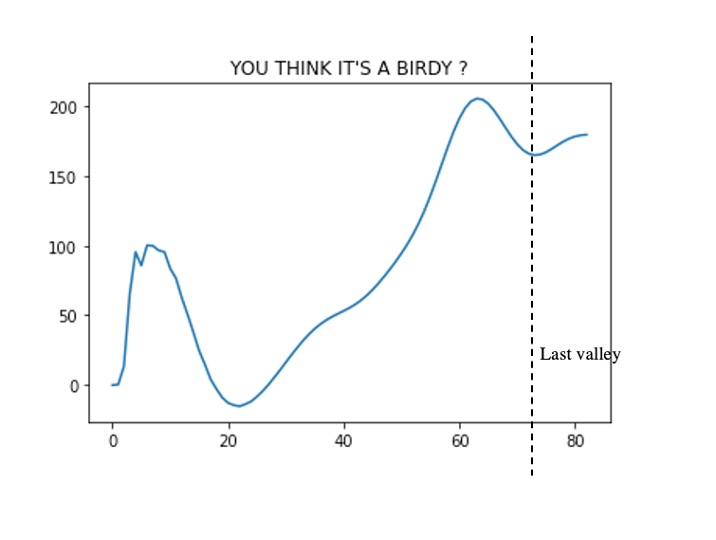
\includegraphics[width=0.7\textwidth]{figures/pitch-rise.jpg}
    \caption{``You think it's a birdy?''}
    \label{fig:rise-example}
\end{figure}

Figure~\ref{fig:rise-sp} and \ref{fig:rise-cl} show the proportion of final rise, as identified by the algorithm. As we can see, there is no difference in the proportion of rises among speech acts. 

\begin{figure}[H]
    \centering
    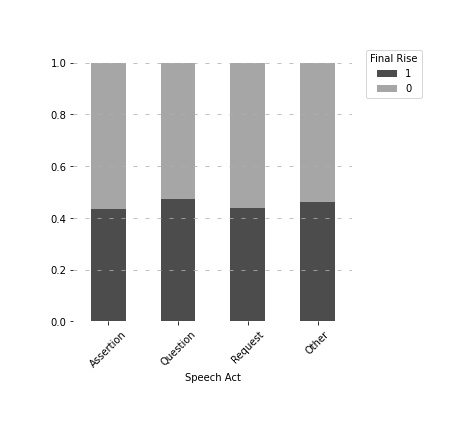
\includegraphics[width=0.7\textwidth]{figures/rise-sp.jpg}
    \caption{Proportion of utterances with final rise across different speech acts}
    \label{fig:rise-sp}
\end{figure}


\begin{figure}[H]
    \centering
    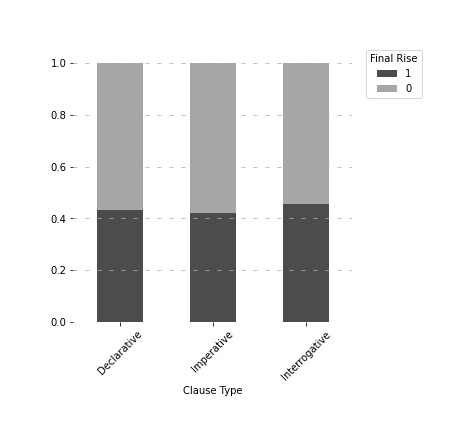
\includegraphics[width=0.7\textwidth]{figures/rise-cl.jpg}
    \caption{Proportion of utterances with final rise across different clause types}
    \label{fig:rise-cl}
\end{figure}

But if we look into sub-categories of interrogatives, we can see that the proportion of final rise is much higher with polar interrogatives than with declaratives. 
\begin{figure}[H]
    \centering
    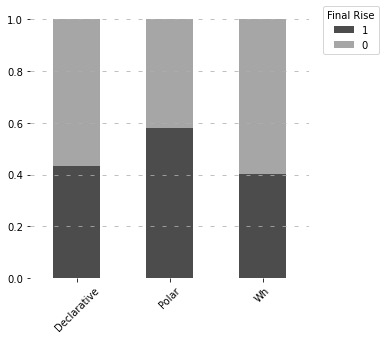
\includegraphics[width=0.7\textwidth]{figures/pitch-polardecwh.jpg}
    \caption{Proportion of declaratives, \twh{} and polar interrogatives with final rise}
    \label{fig:rise-int}
\end{figure}

These results seem to suggest that the presence of final rise might not be informative of the speech act of the sentence, unless morpho-syntactic features like subject-auxiliary inversion is also present. However, this could be a result of the algorithm I applied here, and do not reflect the pattern of the data. I plan to hand annotate more cases in the future to have more reliable data.

\section{Learning clause type categories with prosody}\label{sec:prosody:model}


\begin{minipage}[b]{0.45\linewidth}
\begin{figure}[H]
\begin{center}
\begin{tikzpicture}
\node[latent] (c) {$C_{i}$};
\node[obs, below=of c, xshift=-0.6cm] (s) {$\vec{S_{i}}$};
\node[obs, below=of c, xshift=0.6cm] (i) {$I_{i}$};
\node[latent, right=of i] (lambda) {$\lambda^{c}$};
%\node[const, right=of lambda] (eta) {$\eta$};
\node[latent, right=of c] (phi) {$\phi$};
%\node[const, right=of phi] (beta) {$\beta$};
\node[latent, left=of s] (delta) {$\delta^{(c)}$};
%\node[const, left=of delta] (gamma) {$\gamma$};


\edge {phi}{c};
\edge {c}{s};
\edge {delta}{s};
%\edge {beta}{phi};
%\edge {gamma}{delta};
\edge {lambda, c}{i};
%\edge {eta}{lambda};


\plate {nutt}{(c)(s)(i)}{$N$};
\plate {cvalue}{(delta)}{$C$};
\plate {fvalue}{(cvalue)(s)}{$F$};
%\plate {fvalue}{(gamma)(delta)(s)(cvalue)}{$F$};
\end{tikzpicture}
\end{center}
%\caption{Hierarchical model with all parameters specified}\label{fg:model}
\end{figure}
\end{minipage}
\hspace{0.6cm}
\begin{minipage}[b]{0.45\linewidth}
\begin{figure}[H]
\begin{center}
\begin{tikzpicture}
\node[obs] (a) {$A_{i}$};
\node[latent, right=of a] (theta) {$\theta$};
%\node[const, right=of theta] (alpha) {$\alpha$};
\node[latent, below=of a] (c) {$C_{i}$};
\node[obs, below=of c, xshift=-0.6cm] (s) {$\vec{S_{i}}$};
\node[obs, below=of c, xshift=0.6cm] (l) {$I_{i}$};
\node[latent, right=of l] (lambda) {$\lambda^{c}$};
%\node[const, right=of lambda] (eta) {$\eta$};
\node[latent, right=of c] (phi) {$\phi^{(a)}$};
%\node[const, right=of phi] (beta) {$\beta$};
\node[latent, left=of s] (delta) {$\delta^{(c)}$};
%\node[const, left=of delta] (gamma) {$\gamma$};

\edge {theta}{a};
%\edge {alpha}{theta};
\edge {phi, a}{c};
\edge {delta, c}{s};
%\edge {beta}{phi};
%\edge {gamma}{delta};
\edge {c,lambda}{l};
%\edge {eta}{lambda};


\plate {nutt}{(a)(c)(s)(l)}{$N$};
\plate {avalue}{(phi)}{$A$};
\plate {cvalue}{(delta)}{$C$};
\plate {fvalue}{(delta)(s)(cvalue)}{$F$};
\end{tikzpicture}
\end{center}
%\caption{Hierarchical model with all parameters specified}\label{fg:model}
\end{figure}
\end{minipage}

\begin{equation}\label{postC}
\begin{split}
p(c_{i}| c_{-i}, \vec{a}, \beta, \vec{S_{i}}, \delta, \gamma, l_{i}, \lambda, \eta) = &
\frac{p(\vec{S_{i}}| \vec{c}, \delta, \gamma)\ p(l_{i} |\vec{c},\lambda, \eta)\ p(c_{i}|\beta, c_{-i}, \vec{a})}{\Sigma_{c_{i}'}p(\vec{S_{i}}| \vec{c'}, \delta, \gamma)\ p(l_{i} |\vec{c'},\lambda, \eta)\ p(c_{i}'|\beta, c_{-i}, \vec{a})}\\
=& \frac{ \prod_{F}\frac{\gamma_{0}+n_{s^{F, c_{i}}_{i}}}{2r_{0}+n_{c^{F}_{i}}}%S
\frac{\eta_{0}+n_{l_{i}}^{c_{i}}}{2\eta_{0}+n_{c_{i}}}%L
\frac{\beta_{0}+n_{c_{i}}^{a_{i}}}{4\beta_{0}+n_{a_{i}}}%C
}%分子
{\sum_{c'_{i}}\prod_{F}\frac{\gamma_{0}+n^{F, c'_{i}}_{s_{i}}}{2r_{0}+n^{F}_{c'_{i}}}%S
\frac{\eta_{0}+n_{l_{i}}^{c'_{i}}}{2\eta_{0}+n_{c'_{i}}}%L
\frac{\beta_{0}+n_{c'_{i}}^{a_{i}}}{4\beta_{0}+n_{a_{i}}} %C
}%分母
\end{split}
\end{equation}

The data for this model were taken from the annotated dataset reported in Section~\ref{sec:engcl:corpus}. The labels of speech acts and morpho-syntactic observations were used as input to the models, and the true labels of clause type were used to evaluate the performance of the models. As the learners need to use the surface features of sentences to learn about clause-level properties, instead of one-noun utterances or utterances of only injectives, we eliminated from the dataset sentences that do not contain a verb or an auxiliary. In total, $3366$  sentences were fed into the models.


Overall, the \dlearnerabbr{} model fails to identify the clause type clustering in English, and fails to identify the characteristic morpho-syntactic properties for these clause types. 

\revise{Zooming in on the clusters identified by the models, I found that simulations with around 80\% noise cannot successfully identify all three clusters correctly while simulations with 70\% noise level can, even though the adjusted rand scores of these two levels are roughly the same. At 80\%, we can see that the \plearnerabbr{} reverts back to the performance of the \dlearnerabbr{} in that it fails to identify a cluster for declaratives (Figure~\ref{fig:heatmap-prosody}). Similar to the \dlearnerabbr{} model, the cluster containing most imperatives also contains many declaratives (\ref{fig:heatrev-prosody}). }

\begin{figure}[H]
\begin{minipage}[b]{0.45\linewidth}	
    \centering
    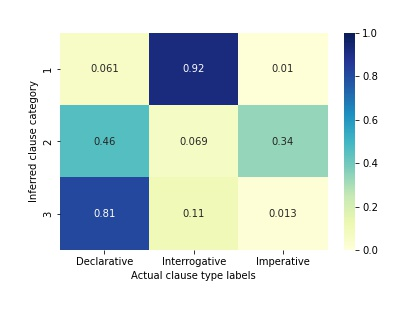
\includegraphics[width=1.2\textwidth]{figures/baseline-heatmap-bu.jpg}
\end{minipage}
\begin{minipage}[b]{0.45\linewidth}	
\centering
    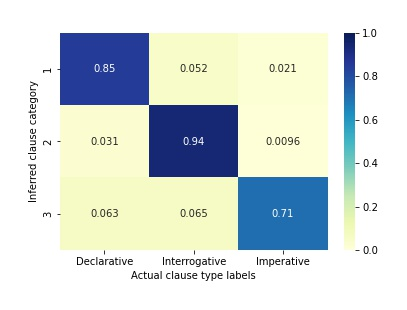
\includegraphics[width=1.2\textwidth]{figures/target-heatmap-bu.jpg}
\end{minipage}
    \caption{The proportion of \diis{} in each of the three clusters identified by the \dlearnerabbr{} (left) and the \plearnerabbr{} model (right). }
    \label{fig:heatmap-prosody}
\end{figure}

\begin{figure}[H]
\begin{minipage}[b]{0.45\linewidth}	
    \centering
    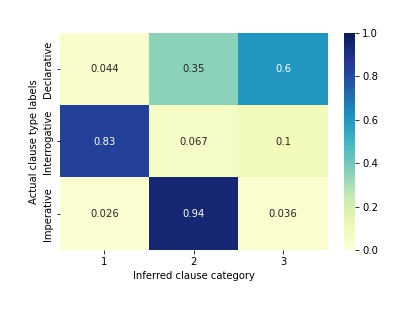
\includegraphics[width=1.2\textwidth]{figures/baseline-heatrev-bu.jpg}
\end{minipage}
\begin{minipage}[b]{0.45\linewidth}	
    \centering
    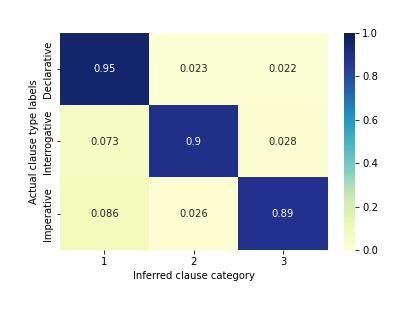
\includegraphics[width=1.2\textwidth]{figures/target-heatrev-bu.jpg}
\end{minipage}   
    \caption{The proportion of actual \diis{} clustered in one category as identified by the \dlearnerabbr{} (right) and \plearnerabbr{} (left) model with prosody respectively}
    \label{fig:heatrev-prosody}
\end{figure}



\revise{The morpho-syntactic profile of different simulations further shows that at 80\% noise level, the \plearnerabbr{} and \dlearnerabbr{} model behave similarly, as both fail to identify the property [$-$ subject] for imperatives (Figure~\ref{fig:noisy80-syncluster}). In contrast, with 70\% noise level the model can still find the right morpho-syntactic features for interrogatives and imperatives (Figure~\ref{fig:noisy70-syncluster}).} 

\begin{figure}[H]
    \centering
    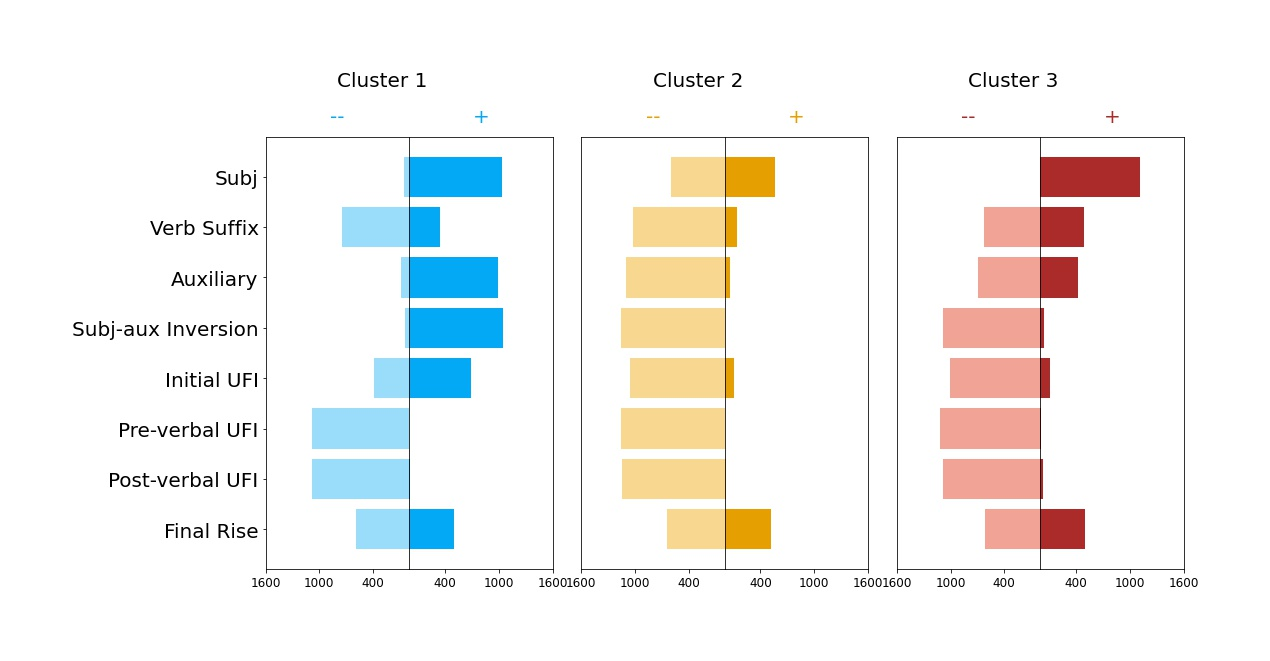
\includegraphics[width=1\textwidth]{figures/baseline-syncluster-bu.jpg}
    \caption{\revise{The morpho-syntactic profile of each cluster in simulations (Cluster 1 $\sim$ Imperatives, Cluster 2 $\sim$ Interrogatives, Cluster 3 $\sim$ Declaratives).}}
    \label{fig:baseline-syncluster-prosody}
\end{figure}

\begin{figure}[H]
    \centering
    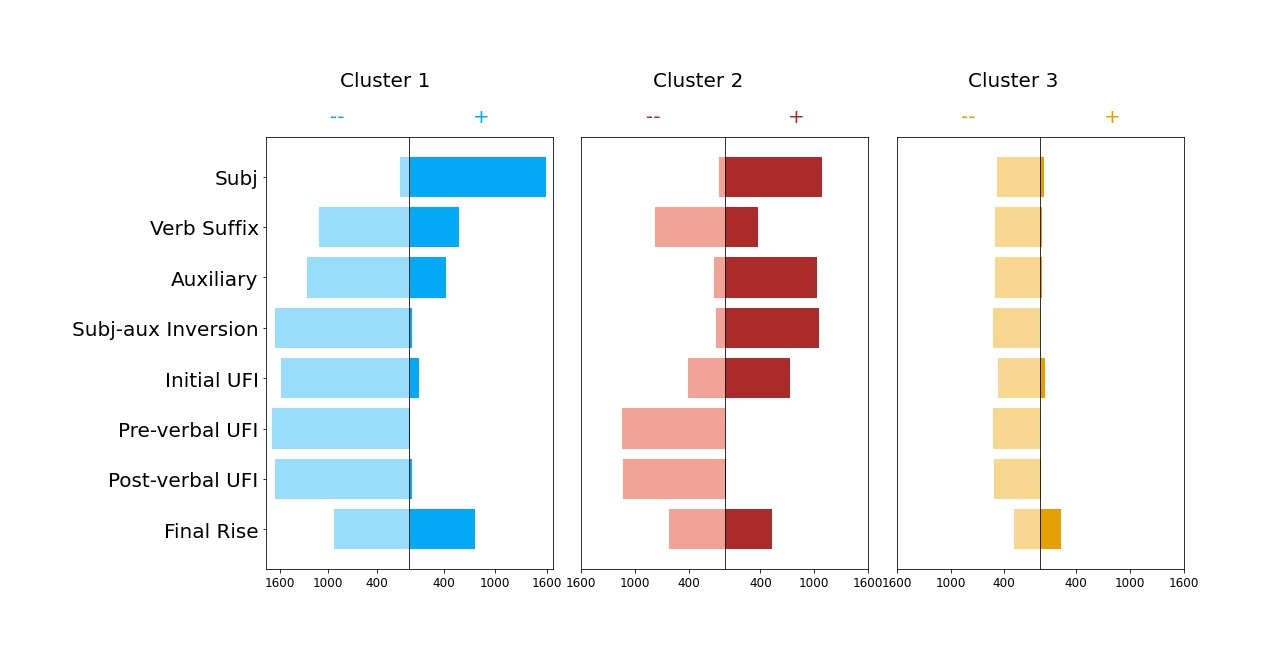
\includegraphics[width=1\textwidth]{figures/target-syncluster-bu.jpg}
    \caption{\revise{The morpho-syntactic profile of each cluster in simulations with 70\% noise in speech act information (Cluster 1 $\sim$ Interrogatives, Cluster 2 $\sim$ Imperatives, Cluster 3 $\sim$ Declaratives).}}
    \label{fig:target-syncluster-prosody}
\end{figure}

Results from our simulations suggest that morphosyntax is not sufficient to solve the clustering problem, and a small amount of pragmatic information is necessary.


\section{Conclusion}
\label{sec:prosody:discussion}
Cross-linguistically, pitch rises tend to signal questions and pitch falls signal assertions; and some argue that this universality reflects the innate knowledge that high pitch connects to the speech act of questioning (\cite{ohala1984,gussenhovenchen2000,gussenhoven2002} among others). If children are armed with the knowledge that questions tend to be associated with rising contours, they might expect rising contours to be somewhat correlated with the act of asking a question. But just as not all interrogatives have subject-auxiliary inversion, not all questions have final rises. With preliminary data, I found that parents do not use final rises more often with questions, but polar interrogatives have more final rises than other types of speech acts and clause types, including \twh-interrogatives and declaratives. It is hard to make sense of how children could take advantage of the prosodic data, since the correlation between final rise is not with the questioning speech act, but with a specific type of interrogative. 

